\chapter{Methodology}
\label{cha:methodology}

In order to estimate the theoretical bitcoin mining performance, the performance
of the hashing accelerator is measured both when using a DMA for data transfer
and without a DMA. The results are compared to a software implementation of the
algorithm.

In addition to measuring the hashing performance, the power efficiency of the
solution is evaluated, allowing estimating the number of hashes per W, a number
that can be compared with other hardware.

\section{Test Setup}
\label{sec:SHMAC_setup}

To test the accelerator, a 20~tile setup was used on SHMAC. A 5x4 grid containing the following
tiles were synthesized, resulting in the following setup, also illustrated in figure \ref{fig:5x4}:

\begin{itemize}
    \item 16 CPU tiles with on-tile DMA and SHA256 accelerator
    \item 2 scratchpad tiles
    \item 1 DRAM tile
    \item 1 I/O tile
\end{itemize}

\todo{Figure \ref{fig:5x4} should change away from T. Should also number each T-tile for ID.}

\begin{figure}[ht]
    \centering
    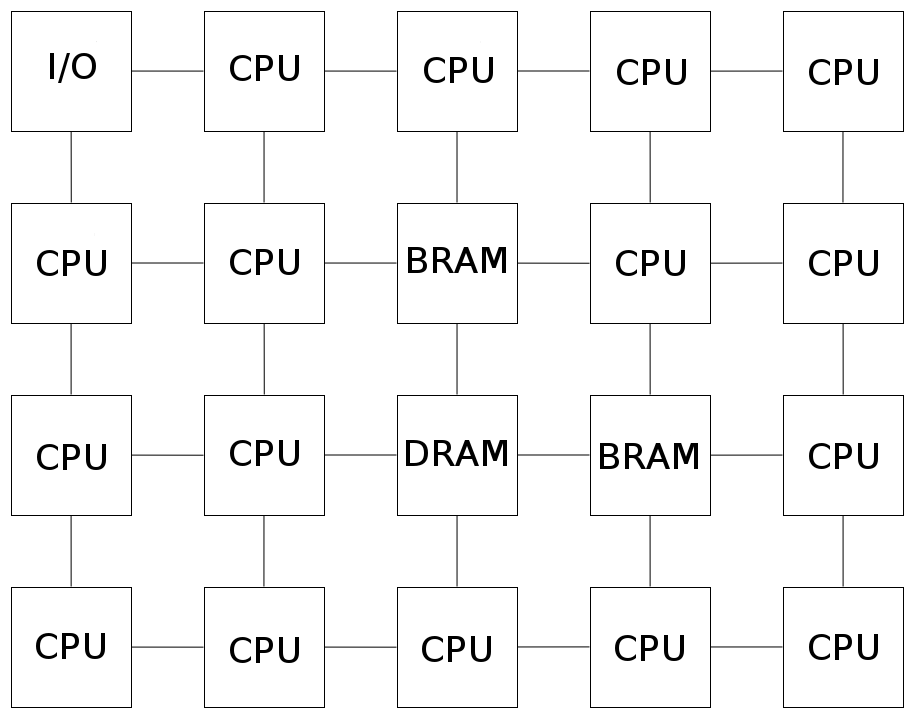
\includegraphics[width=0.5\textwidth]{Figures/Measurements/5x4}
    \caption{Test setup: T are Turbo Amber tiles, R are scRathpads, D is the DRAM tile and V is the I/O interface.}
    \label{fig:5x4}
\end{figure}

\section{Measuring the Performance}

Measuring the performance is done by repeatedly hashing a block of data, recording the
number of hashes achieved per second per core. By turning on one core at a time, it
is possible to see how the performance scales as more cores are added, and recording
the number of hashes per second per core makes it possible to see how the performance
of each core is affected by the traffic generated by the other cores in the network
between the tiles.

Using the setup described in section \ref{sec:SHMAC_setup}, tests where run using the
following method:

\begin{itemize}
    \item Hashing using software only, not using the SHA256 hashing module or DMA module.
    All work is done by the on-tile processor.
    \item Hashing using only the hashing accelerator.
    The processor controls and copies data to and from the hashing module.
    \item Hashing using the hashing accelerator and DMA.
    The processor controls each module, but the DMA handles data transfer.
\end{itemize}

Interrupts are used by the hashing module to signal when it is finished working. However,
the DMA does not support interrupts and has to be polled while copying data to and from
the module, which may influence the results.

\section{Measuring Power Usage}

Power usage for the application is determined by measuring the wall-power of the box
that SHMAC is running on both when idle and when running the test applications:

\[P_{application} = P_{running} - P_{idle}\]


% WARNING: Mathematical symbols are always explained bit by bit in most papers I have read. And we should explain why we chose this way (lack of counters on-chip)

% NOTE TO SELF: At some point, I think we need to underline the existing problems (cache bug, cache coherency issues, etc.), in order to affirm whenever they affect our test results.
% Furthermore, a report should always provide the means for the results to be reproduced.
% Must discuss with Kristian.

% FOLLOWING POST-MEETING:

\section{SHMAC Throughput}
\textbf{Optional position: Chapter 3 describing SHMAC}
Write here the numbers from shmac: Expected tile-to-tile routing time, Max throughput on DRAM-access, etc.etc. Anything we know that may impact our testing of the bitcoin mining

Optional: Write the expected max performance if we can calculate them?

\section{Known hazards with SHMAC}
List up potential problems that SHMAC may give us, due to the known bugs in the system (cache coherency issues with DMA, the infamous cache bug



%\section{Test benchmark}
%
%Caches were turned on for each testing, but a bug in the caches can cause several processors to halt over time, making measurements more difficult.
%Increased number of tiles in used increases the chance for a cache bug to happen.
%Additionally, no cache coherency protocol is implemented, and all shared data are therefore mapped to uncachable memory.
%Data hazard may be present when DMA and processor "shares" data, by loading or storing to the same address space in use.
%DMA may copy outdated data from memory that the cache has not yet written back, or overwrite data that the cache is not aware of.
%An operating system may handle data coherency where DMA involved, but since this project is done by running the software on bare metal, this security is absent.
%The Turbo Amber processor uses \todo{Must get it confirmed, and then source linked}write-through policy, so every data update is always written back to memory, \todo{Want to mention "reduced, but not removed", due to how our tests may go} reducing the possibility of data hazard, but not removing it.

%Interrupt handling for the hashing module is always in use, when the accelerator is used.

%The DMA Module is made only for transfering 32-bit words individually at a time.
%When transferring data internal on the tile (regular tile registers, hashing registers and DMA registers), this is all the local system requires, as the tile modules does not provide full blocks of \todo{Use of wishbone, with size 128, is not yet provided}4 words.
%\todo{Merely an assumption. We haven't tested this.}But when running the hashing in software only, the system is likely to achieve better data transfer rate using regular processor data transfer of 4 words, through the caches, since the current DMA would require 4 individual transfer, compared to the processor.

%The use of the included sub-module in the DMA that moves the bytes from high endian to little endian should further improve the performance and energy efficiency, by relieving the software for this task.
%The byte flip is done through combinatorical circuits, and should not add any extra execution time.
%Wihtout it, the software would require several independent operations, for loading in and shifting every single byte to the correct position of the word.

%Additionally, polling is used to control when a DMA is finished.
%Ideally, interrupt handling is preferable, but the interrupt handler for the DMA would not \todo{yet}work. 
